\chapter{Phân tích thiết kế hệ thống}
\label{chapter3}
Từ những cơ sở lý thuyết thu thập ở chương \ref{chapter2}, chương \ref{chapter3} em sẽ trình bày phân tích yêu cầu chức năng quy trình thiết kế hệ thống.
\section{Phân tích yêu cầu}
\subsection{Mô tả hệ thống}
Một website thương mại cho phép cửa hàng có thể bán tất cả các loại mặt hàng, có thể giao dịch trực tuyển qua nhiều hinhf thức thanh toán như là: Ngân Lượng, Bảo Kim, ATM, COD,...
Chủ đạo của website là đăng thông tin sản phẩm thật cho khách hàng dễ dàng tìm kiểm thông qua mạng Internet rất phổ cập hiện nay. Người quản trị chính là chủ cửa hàng có một trang quản trị riêng đẻ đăng những thông tin sản phầm, quản lý hoá đơn mua hàng, xem doanh thu theo những mốc thời gian mà người quản trị cần, quản lý thông tin cửa hàng, quản lý quyền cho hệ thống cũng như những tài khoản của khách hàng và cho phép cửa hàng có thể bán thêm những mặt hàng mới nên sẽ phải có hệ thống danh mục sản phầm động. Để thuận tiện cho người quản lý phải có thêm chức năng tìm kiếm ở mỗi chức năng quản lý.
\par
Đối với khách hàng họ cần có 1 tài khoản với thông tin chính xác đề người quản trị liên hệ lại với họ và tiền hành giao dịch mua bán. Với trang chủ để khách hàng xem thông tin sản phẩm chúng ta cần phải có 1 giao diện bắt mắt và thân thiện với người dùng kèm theo đấy là những chức năng tìm kiếm theo những điều kiện khác nhau để người dùng có thể xem những sản phầm họ cần thật nhanh. Vì đây là 1 trang web thương mại điện tử chúng ta không thể thiếu đi được chức năng đăng ký đăng nhập cũng như thay đổi các thông tin cá nhân liên quan đến tài khoản người dùng. Một điều quan trọng hơn nữa là phải lưu được hoá đơn kèm theo đối với mỗi tài khoản người dùng và hỗ trợ chức năng thêm nhiều sản phẩm vào giỏ hàng để người sử dụng dễ dàng hơn trong việc mua sắm.
\subsection{Yêu cầu hệ thống}
\subsubsection{Yêu cầu chức năng}
 Hệ thống website thương mại điện tử sẽ được chia theo nhiều cấp độ người dùng:
\begin{itemize}
 \item Người quản trị: Có mọi quyền để tương tác trong hệ thống, người quản trị có thể thay đối bất kì thông tin của sản phẩm hay đăng bài viết của cửa hàng mình lên tràng chủ, người quản lý có thêm thêm nhân viên giao hàng vào các đơn hàng mà phương thức vận chuyển là COD, người quản lý có thể xem doanh thu bán hàng.  
 \item Nhân viên quản lý của hàng: Chỉ có thế xem và sửa thông tin các sản phầm để cập nhật nhanh chóng lên trang chủ phục vụ nhu cầu của khách hàng.
 \item Người vận chuyển hàng: Chỉ được xem hoá đơn theo trạng thái COD và vận chuyển hàng theo đơn hàng đã được giao trong hệ thống.
 \item Khách hàng: Khách hàng chỉ được phép truy cập ở trang chủ còn trang quản trị thì họ không có quyền gì, khách hàng có thể đăng kí, đăng nhập, và thay đổi thông tin tài khoản để mua hàng, họ cũng có thể gửi những đóng góp cho người quản trị để phát triền website hơn nữa.
\end{itemize}  
\subsubsection{Yêu cầu phi chức năng}
Ngoài các yêu cầu chức năng hệ thống còn có những yêu cầu phi chức năng sau:
\begin{itemize}
\item Hệ thồng có dung lượng không quá lớn, tốc độ xử lý nhanh hơn.
\item Công việc thực hiện chính xác.
\item Sử dụng mã hoá các thông tin nhạy cảm của khách hàng như: mật khẩu, ngày sinh nhật, số điện thoại,...
\item Đảm bảo an toàn dữ liệu khi chạy website trực tuyến
\end{itemize}
\section{Thiết kế hệ thống}
\subsection{Sơ đồ tổng quan hệ thống}
Hệ thống website bao gồm:
\begin{itemize}
    \item Cơ sở dữ liệu là một tập hợp những thông tin được tổ chức để dễ dàng trong việc tạo lập, cập nhập và khai thác thông tin. Cơ sở dữ liệu được duy trì dưới dạng một tập hợp các tập tin trong hệ điều hành hay được lưu trữ trong các hệ quản trị cơ sở dữ liệu. Cơ sở dữ liệu được phân chia thành nhiều loại khác nhau:
   \begin{itemize}
   \item Cơ sở dữ liệu dạng file: dữ liệu được lưu trữ dưới dạng các file có thể là text, ascii,...
   \item Cơ sở dữ liệu quan hệ: dữ liệu được lưu trữ trong các bảng dữ liệu gọi là các thực thể, giữa các thực thể này có mối liên hệ với nhau gọi là các quan hệ, mỗi quan hệ có các thuộc tính, trong đó có một thuộc tính là khóa chính. Các hệ quản trị hỗ trợ cơ sở dữ liệu quan hệ như: MS SQL server, Oracle, MySQL...
   \item Cơ sở dữ liệu hướng đối tượng: dữ liệu cũng được lưu trữ trong các bảng dữ liệu nhưng các bảng có bổ sung thêm các tính năng hướng đối tượng như lưu trữ thêm các hành vi, nhằm thể hiện hành vi của đối tượng. Mỗi bảng xem như một lớp dữ liệu, một dòng dữ liệu trong bảng là một đối tượng. Các hệ quản trị có hỗ trợ cơ sở dữ liệu hướng đối tượng như: MS SQL server, Oracle, Postgres
   \item Cơ sở dữ liệu bán cấu trúc: dữ liệu được lưu dưới dạng XML, với định dạng này thông tin mô tả về đối tượng thể hiện trong các tag. Đây là cơ sở dữ liệu có nhiều ưu điểm do lưu trữ được hầu hết các loại dữ liệu khác nhau nên cơ sở dữ liệu bán cấu trúc là hướng mới trong nghiên cứu và ứng dụng.
   \item Cơ sở dữ liệu phân cấp (blockchain): Dữ liệu được phân tán trên mạng máy tính ngang hàng và luôn được cả mạng lưới kiểm định. Ví dụ: Bitcoin blockchain.
   \end{itemize}
    \item Trang quản trị bao gồm các công việc liên quan đến xử lý nội dung, hình ảnh và các vấn đề phát sinh trong quá trình sử dụng như chữa lỗi, bảo mật, sao lưu và phục hồi thông tin.
    \item Trang chủ website, hiện nay có 2 loại trang chủ website là: 
    \begin{itemize}
    \item Website tĩnh là website mà người quản trị (những người không phải là lập trình viên) không thể tùy ý thay đổi nội dung và hình ảnh mà phải cần kiến thức về HTML cơ bản. Website tĩnh được viết hoàn toàn dựa trên nền tảng HTML CSS và thêm các hiệu ứng từ Javascript nếu muốn.
    \item Website động là website được viết kèm theo một bộ công cụ quản trị để tùy biến nội dung dành cho webmaster (người quản trị) có thể dễ dàng thay đổi nội dung, hình ảnh. Website động được thiết kế bởi các lập trình viên để làm sao cho phép website có thể thay đổi được nội dung thường xuyên. Một số công nghệ, ngôn ngữ để xây dựng website động bao gồm PHP, ASP.NET, Java,...
    \end{itemize}
\end{itemize}
\begin{center}
    \begin{figure}[h]
    \begin{center}
     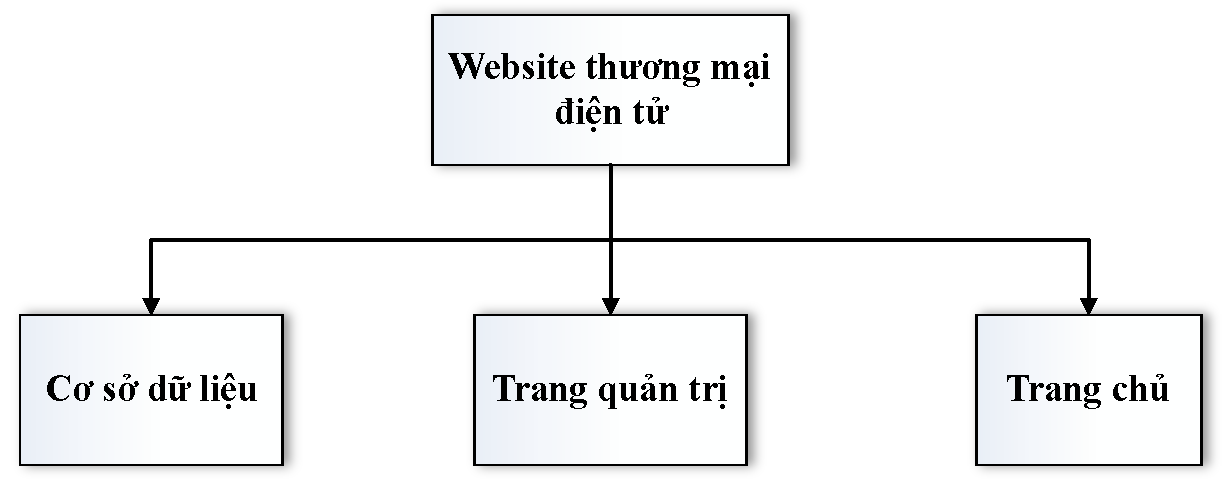
\includegraphics[scale=0.7]{image/TongQuanHeThong.pdf}
    \end{center}
    \caption{Tổng Quan Hệ thống}
    \label{refhinh3_1}
    \end{figure}
\end{center}
\subsection{Sơ đồ Use case diagram}
Một biểu đồ Use case chỉ ra một số lượng các tác nhân ngoại cảnh và mối liên
kết của chúng đối với Use case mà hệ thống cung cấp. Một Use case là một lời miêu tả của một chức năng mà hệ thống cung cấp. Lời miêu tả Use case thường là một văn bản tài liệu, nhưng kèm theo đó cũng có thể là một biểu đồ hoạt động. Các Use case được miêu tả duy nhất theo hướng nhìn từ ngoài vào của các tác nhân (hành vi của hệ thống theo như sự mong đợi của người sử dụng), không miêu tả chức năng được cung cấp sẽ hoạt động nội bộ bên trong hệ thống ra sao. Các Use case định nghĩa các yêu cầu về mặt chức năng đối với hệ thống.
\subsubsection{Quản Trị Viên}
Quản trị viên có vai trò cao nhất trong hệ thống có thể truy cập bất cứ chức năng gì trong hệ thống. Quản trị viên có những chức năng sau:
\begin{itemize}
 \item Tạo ra tài khoản cho các cấp người dùng.
 \item Tạo ra các quyền và nhóm quyền sau đó gán cho người dùng tương ứng.
 \item Thêm, sửa, xoá, xem thông tin sản phẩm, danh mục sản phẩm, hoá đơn bán hàng, người vận chuyển, những quảng cáo trên website, góp ý khách hàng, thông tin của cửa hàng.
 \item Khoá một tài khoản của người dùng.
 \item Xem doanh thu của cửa hàng.
 \item Gửi mail cho người dùng sau khi người dùng đăng kí tài khoản.
 \item Được xem hiển thị thông báo mỗi khi hệ thống có sự thay đổi như: thêm mới, sửa, xoá, hay có một đơn hàng mới.
 \end{itemize}
\newpage
 \begin{center}
    \begin{figure}[h]
    \begin{center}
     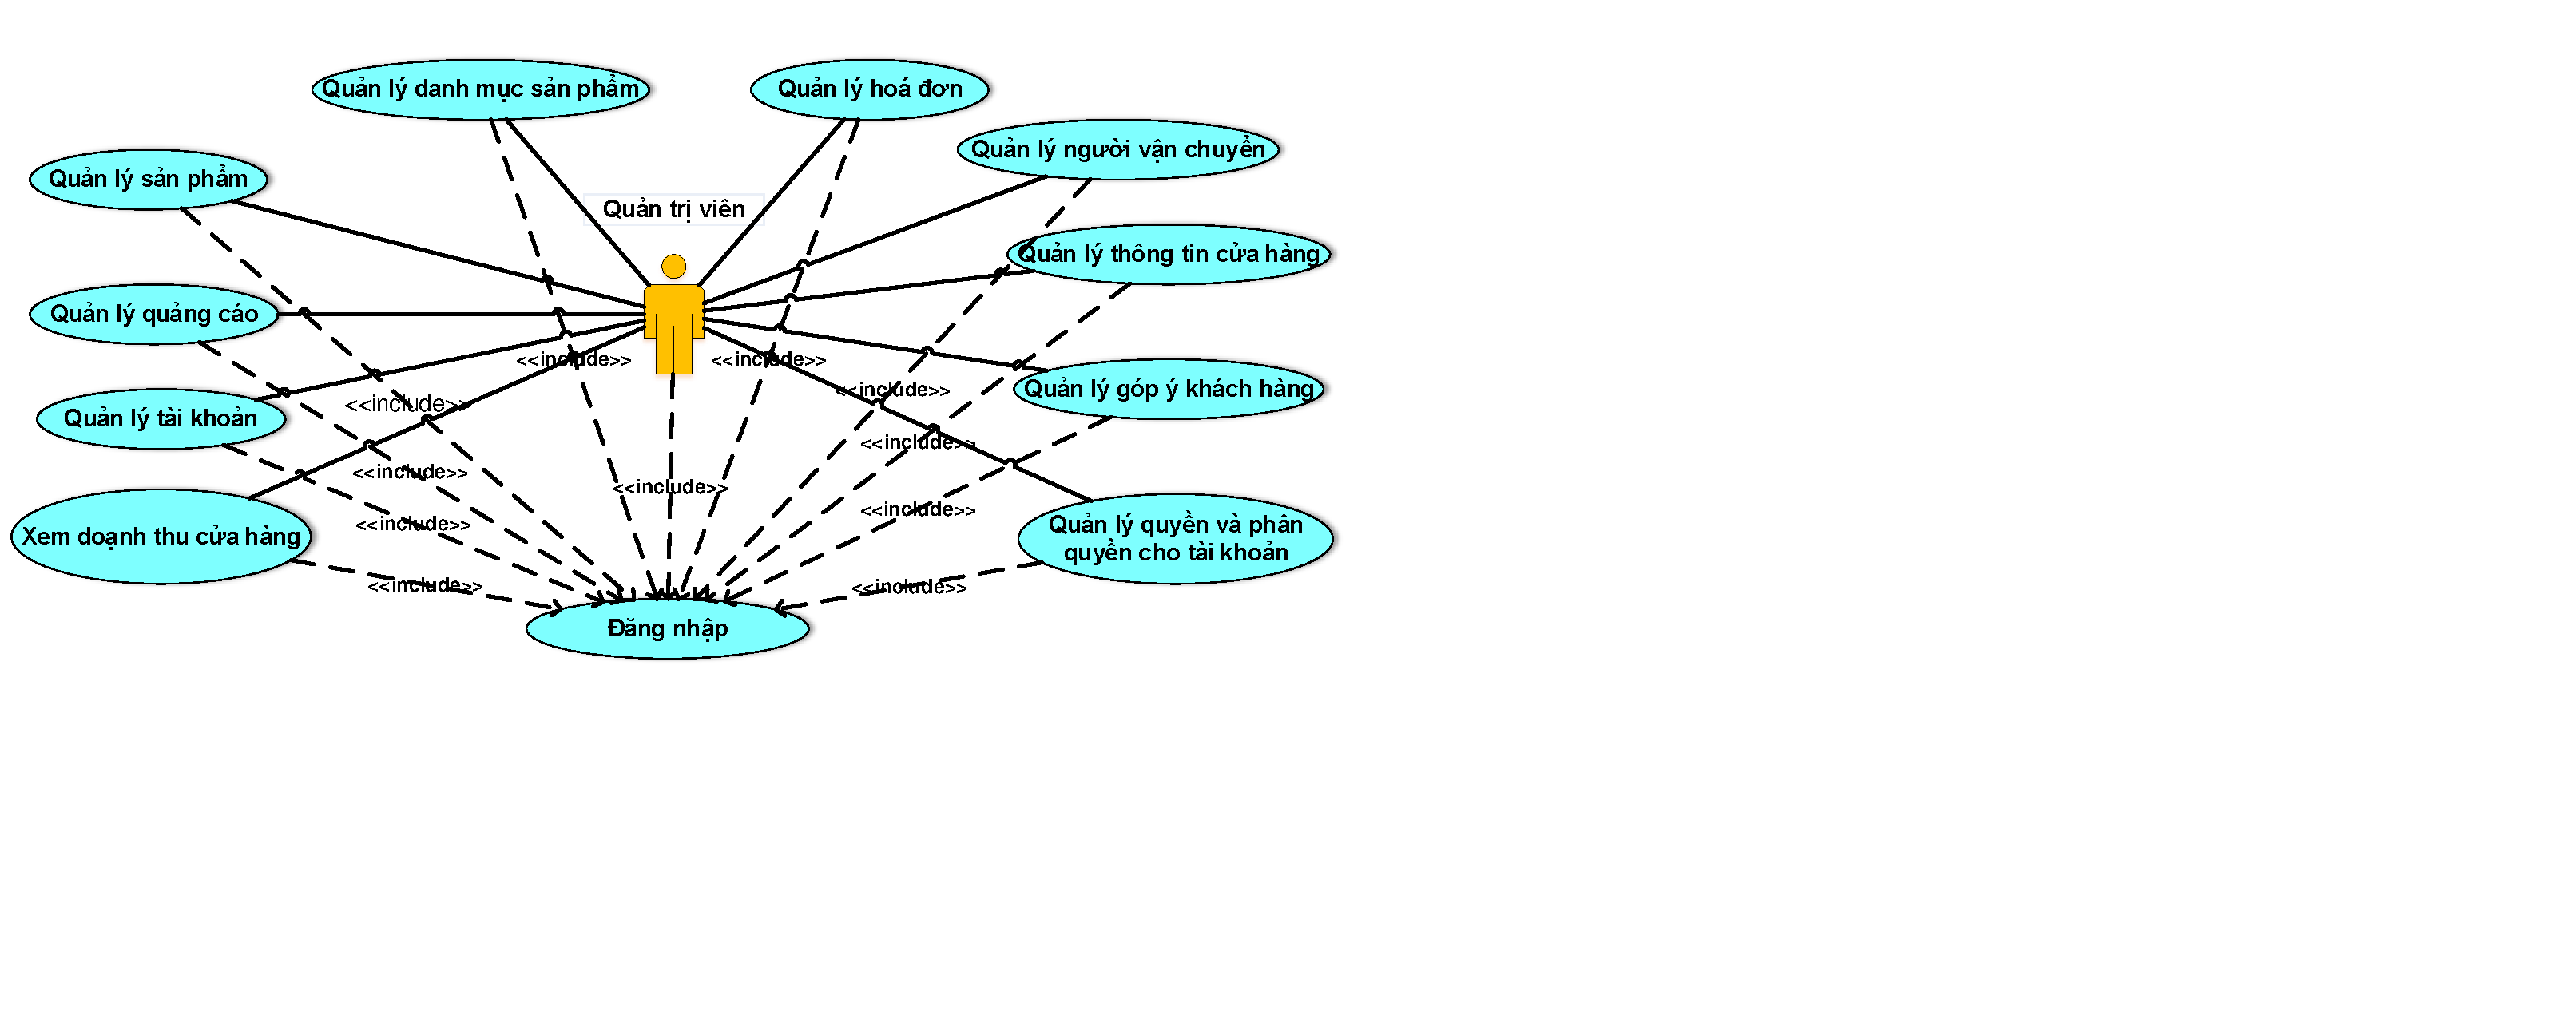
\includegraphics[scale=0.5]{image/UseCaseTongQuanQTV.pdf}
    \end{center}
    \caption{Use-Case Quản Trị Viên}
    \label{refhinh3_2}
    \end{figure}
\end{center}
Từ Hình \ref{refhinh3_2} ta có các bảng đặc tả chi tiết cho các Use-Case của quản trị viên:
- Use-Case đăng nhập:
\begin{longtable}[htp]{ |m{0.25\linewidth}|m{0.65\linewidth}|}
 \caption{Bảng Use-Case đăng nhập \label{login}}\\
 \hline
 Use-Case & Nội dung \\
 \hline
 Tên Use-Case & Đăng nhập \\
 \hline
 Mô tả & Use-case cho phép quản trị viên đăng nhập vào hệ thống để thực hiện những chức năng của mình\\
 \hline
 Tên tác nhân & Quản trị viên\\
 \hline
 Điều kiện kích hoạt & Quản trị viên vào trang admin trên hệ thống, trang admin bắt buộc phải đăng nhập\\
 \hline
 Tiền điều kiện & Quản trị viên phải có tài khoản trên hệ thống và được phân quyền quản trị viên\\
 \hline
 Hậu điều kiện & Quản trị viên đăng nhập thành công\\
 \hline
 Luồng sự kiện chính & 
  1. Hệ thống hiện thị màn hình đăng nhập.\newline
  2. Quản trị viên nhập tên đăng nhập và mật khẩu.\newline
  3. Hệ thống kiểm tra thông tin đăng nhập và kiểm qua quyền của tài khoản là admin.\newline
  4. Nếu thành công hệ thống sẽ đưa quản trị viên vào trang chủ của trang quản trị.\newline
  5. Kết thúc Use-case.	
 \\
 \hline
 Luồng sự kiện phụ & 
 - Tài khoản và mật khẩu không hợp lệ:\newline
 1. Khi quản trị viên nhập sai tên đăng nhập và mật khẩu\newline
 2. Hệ thống hiển thị lại màn hình đăng nhập để quản trị viên nhập lại thông tin tài khoản và mật khẩu kèm theo thông báo tên đăng nhập và mật khẩu bị sai.\newline
  Quay lại bước 2 trong luồng sự kiện chính.
 \\
 \hline
\end{longtable}
\par
- Use-Case Đăng xuất:

\begin{longtable}[htp]{ |m{0.3\linewidth}|m{0.6\linewidth}|}
 \caption{Bảng Use-Case đăng xuất \label{logout}}\\
 \hline
 Use-Case & Nội dung \\
 \hline
 Tên Use-Case & Đăng xuất \\
 \hline
 Mô tả & Use-case cho phép quản trị viên đăng xuất ra khỏi hệ thống\\
 \hline
 Tên tác nhân & Quản trị viên\\
 \hline
 Điều kiện kích hoạt & Quản trị viên nhấn nút đăng xuất trên màn hình hệ thống\\
 \hline
 Tiền điều kiện & Quản trị viên đã đăng nhập vào hệ thống\\
 \hline
 Hậu điều kiện & Quản trị viên đăng xuất thành công\\
 \hline
 Luồng sự kiện chính & 
 1. Quản trị viên tìm và nhấn nút đăng xuất.\newline
 2. Hệ thống xử lý yêu cầu đăng xuất của quản trị viên.\newline
 3. Kết thúc Use-case.	
 \\
 \hline
\end{longtable}

- Use-case quản lý tài khoản:

\begin{longtable}[htp]{ |m{0.3\linewidth}|m{0.6\linewidth}|}
 \caption{Bảng Use-Case thêm mới tài khoản \label{long}}\\
 \hline
 Use-Case & Nội dung \\
 \hline
 Tên Use-Case & Thêm mới tài khoản \\
 \hline
 Mô tả & Use-case cho phép quản trị viên thêm mới tài khoản để cấp cho người dùng sử dụng hệ thống\\
 \hline
 Tên tác nhân & Quản trị viên\\
 \hline
 Điều kiện kích hoạt & Quản trị viên vào trang admin trên hệ thống, chọn chức năng thêm tài khoản\\
 \hline
 Tiền điều kiện & Quản trị viên phải đăng nhập vào hệ thống và có quyền thêm tài khoản\\
 \hline
 Hậu điều kiện & Thông tin tài khoản mới được cập nhật vào cơ sở dữ liệu\\
 \hline
 Luồng sự kiện chính & 
 1. Quản trị viên kích hoạt yêu cầu thêm tài khoản.\newline
 2. Hệ thống hiển thị giao diện thêm tài khoản và yêu cầu quản trị viên nhập thông tin tài khoản.\newline
 3. Quản trị viên nhâp thông tin tài khoản mới và nhấn lưu tài khoản.\newline
 4. Hệ thống kiểm tra thông tin tài khoản và xác nhận hợp lệ.\newline
 5. Hệ thống thông báo đã lưu thành công tài khoản.\newline	
 6. Quản trị viên thoát khỏi chức năng thêm tài khoản
 \\
 \hline
 Luồng sự kiện phụ & 
 - Dữ liệu không đúng:\newline
  1. Hệ thống hiển thị lại giao diện nhập thông tin tài khoản để quản trị viên nhập lại đồng thời hiện thị thông báo lưu tài khoản không thành công.\newline
  2. Quay lại bước 2 của luồng sự kiện chính.\newline
  - Không có quyền thực hiện chức năng:\newline
  1. Hệ thống kiểm tra lúc đăng nhập tài khoản không có quyền thực hiện chức năng.\newline
  2. Trên thanh chức năng không có chức năng thêm tài khoản
 \\
 \hline
\end{longtable}

\begin{longtable}[htp]{ |m{0.3\linewidth}|m{0.6\linewidth}|}
 \caption{Bảng Use-Case sửa tài khoản \label{long}}\\
 \hline
 Use-Case & Nội dung \\
 \hline
 Tên Use-Case & Sửa tài khoản \\
 \hline
 Mô tả & Use-case cho phép quản trị viên sửa tài khoản cho người sử dụng hệ thống\\
 \hline
 Tên tác nhân & Quản trị viên\\
 \hline
 Điều kiện kích hoạt & Quản trị viên vào trang admin trên hệ thống, chọn 1 tài khoản trong danh sách tài khoản\\
 \hline
 Tiền điều kiện & Quản trị viên phải đăng nhập vào hệ thống và có quyền sửa tài khoản\\
 \hline
 Hậu điều kiện & Thông tin tài khoản sau khi sửa được cập nhật vào cơ sở dữ liệu\\
 \hline
 Luồng sự kiện chính & 
 1. Quản trị viên chọn 1 tài khoản.
 2. Quản trị viên kích hoạt yêu cầu sửa tài khoản.\newline
 3. Hệ thống hiển thị giao diện sửa tài khoản và những thông tin tài khoản đã được chọn, yêu cầu quản trị viên sửa tài khoản.\newline
 4. Quản trị viên nhâp thông tin tài khoản mới và nhấn lưu tài khoản.\newline
 5. Hệ thống kiểm tra thông tin tài khoản và xác nhận hợp lệ.\newline
 6. Hệ thống thông báo đã lưu thành công tài khoản.\newline	
 7. Quản trị viên thoát khỏi chức năng sửa tài khoản
 \\
 \hline
 Luồng sự kiện phụ & 
 - Dữ liệu không đúng:\newline
  1. Hệ thống hiển thị lại giao diện nhập thông tin tài khoản để quản trị viên nhập lại đồng thời hiện thị thông báo lưu tài khoản không thành công.\newline
  2. Quay lại bước 2 của luồng sự kiện chính.\newline
  - Không có quyền thực hiện chức năng:\newline
  1. Hệ thống kiểm tra lúc đăng nhập tài khoản không có quyền thực hiện chức năng.\newline
  2. Trên thanh chức năng không có chức năng sửa tài khoảm
 \\
 \hline
\end{longtable}

\begin{longtable}[htp]{ |m{0.3\linewidth}|m{0.6\linewidth}|}
 \caption{Bảng Use-Case xoá tài khoản \label{long}}\\
 \hline
 Use-Case & Nội dung \\
 \hline
 Tên Use-Case & Xoá tài khoản \\
 \hline
 Mô tả & Use-case cho phép quản trị viên xoá tài khoản khi người dùng không sử dụng\\
 \hline
 Tên tác nhân & Quản trị viên\\
 \hline
 Điều kiện kích hoạt & Quản trị viên vào trang admin trên hệ thống, chọn 1 tài khoản trong danh sách tài khoản\\
 \hline
 Tiền điều kiện & Quản trị viên phải đăng nhập vào hệ thống và có quyền xoá tài khoản\\
 \hline
 Hậu điều kiện & Thông tin tài khoản đã chọn được xoá khỏi cơ sở dữ liệu\\
 \hline
 Luồng sự kiện chính & 
 1. Quản trị viên chọn 1 tài khoản.
 2. Quản trị viên kích hoạt yêu cầu xoá tài khoản.\newline
 3. Hệ thống hiển thị giao diện xoá tài khoản và yêu cầu quản trị viên xác nhận có đồng ý xoá không.\newline
 4. Quản trị viên chọn có trên màn hình giao diện.\newline
 5. Hệ thống xoá tài khoản khỏi cơ sở dữ liệu.\newline
 6. Hệ thống thông báo đã xoá thành công tài khoản.\newline	
 7. Quản trị viên thoát khỏi chức năng xoá tài khoản
 \\
 \hline
 Luồng sự kiện phụ & 
 - Không có quyền thực hiện chức năng:\newline
  1. Hệ thống kiểm tra lúc đăng nhập tài khoản không có quyền thực hiện chức năng.\newline
  2. Trên thanh chức năng không có chức năng xoá tài khoảm
 \\
 \hline
\end{longtable}

- Quản lý sản phẩm:
\begin{longtable}[htp]{ |m{0.3\linewidth}|m{0.6\linewidth}|}
 \caption{Bảng Use-Case thêm sản phẩm \label{createProduct}}\\
 \hline
 Use-Case & Nội dung \\
 \hline
 Tên Use-Case & Thêm sản phẩm \\
 \hline
 Mô tả & Use-case cho phép quản trị viên thêm sản phẩm để hiển thị trên trang chủ\\
 \hline
 Tên tác nhân & Quản trị viên\\
 \hline
 Điều kiện kích hoạt & Quản trị viên vào trang admin trên hệ thống, chọn chức năng thêm sản phẩm\\
 \hline
 Tiền điều kiện & Quản trị viên phải đăng nhập vào hệ thống và có quyền thêm sản phẩm\\
 \hline
 Hậu điều kiện & Thông tin sản phẩm sau khi thêm mới được cập nhật vào cơ sở dữ liệu\\
 \hline
 Luồng sự kiện chính & 
 1. Quản trị viên kích hoạt yêu cầu thêm sản phẩm.\newline
 2. Hệ thống hiển thị giao diện thêm sản phẩm và yêu cầu quản trị viên nhập thông tin sản phẩm.\newline
 3. Quản trị viên nhâp thông tin sản phẩm mới bao gồm: giá, tải ảnh sản phẩm, tên sản phẩm,... và nhấn lưu sản phẩm.\newline
 4. Hệ thống kiểm tra thông tin sản phẩm và xác nhận hợp lệ.\newline
 5. Hệ thống thông báo đã lưu thành công sản phẩm.\newline	
 6. Quản trị viên thoát khỏi chức năng thêm sản phẩm.
 \\
 \hline
 Luồng sự kiện phụ & 
 - Dữ liệu không đúng:\newline
  1. Hệ thống hiển thị lại giao diện nhập thông tin sản phẩm để quản trị viên nhập lại đồng thời hiện thị thông báo lưu sản phẩm không thành công.\newline
  2. Quay lại bước 2 của luồng sự kiện chính.\newline
  - Không có quyền thực hiện chức năng:\newline
  1. Hệ thống kiểm tra lúc đăng nhập tài khoản không có quyền thực hiện chức năng.\newline
  2. Trên thanh chức năng không có chức năng thêm sản phẩm.
 \\
 \hline
\end{longtable}

\begin{longtable}[htp]{ |m{0.3\linewidth}|m{0.6\linewidth}|}
 \caption{Bảng Use-Case sửa sản phẩm \label{updateProduct}}\\
 \hline
 Use-Case & Nội dung \\
 \hline
 Tên Use-Case & Sửa sản phẩm \\
 \hline
 Mô tả & Use-case cho phép quản trị viên sửa sản phẩm để hiển thị trên trang chủ\\
 \hline
 Tên tác nhân & Quản trị viên\\
 \hline
 Điều kiện kích hoạt & Quản trị viên vào trang admin trên hệ thống, chọn chức năng sửa sản phẩm\\
 \hline
 Tiền điều kiện & Quản trị viên phải đăng nhập vào hệ thống và có quyền sửa sản phẩm\\
 \hline
 Hậu điều kiện & Thông tin sản phẩm sau khi sửa được cập nhật vào cơ sở dữ liệu\\
 \hline
 Luồng sự kiện chính & 
 1. Quản trị viên chọn 1 trong số sản phẩm cần sửa trong danh sách sản phẩm.
 2. Quản trị viên kích hoạt yêu cầu sửa sản phẩm.\newline
 3. Hệ thống hiển thị giao diện sửa sản phẩm đồng thời hiển thị các thông tin của sản phẩm được chọn và yêu cầu quản trị viên nhập thông tin sản phẩm cần sửa.\newline
 4. Quản trị viên nhâp thông tin sản phẩm mới bao gồm: giá, ảnh sản phẩm, tên sản phẩm,... và nhấn lưu sản phẩm.\newline
 5. Hệ thống kiểm tra thông tin sản phẩm và xác nhận hợp lệ.\newline
 6. Hệ thống thông báo đã lưu thành công sản phẩm.\newline	
 7. Quản trị viên thoát khỏi chức năng sửa sản phẩm.
 \\
 \hline
 Luồng sự kiện phụ & 
 - Dữ liệu không đúng:\newline
  1. Hệ thống hiển thị lại giao diện nhập thông tin sản phẩm để quản trị viên nhập lại đồng thời hiện thị thông báo lưu sản phẩm không thành công.\newline
  2. Quay lại bước 2 của luồng sự kiện chính.\newline
  - Không có quyền thực hiện chức năng:\newline
  1. Hệ thống kiểm tra lúc đăng nhập tài khoản không có quyền thực hiện chức năng.\newline
  2. Trên thanh chức năng không có chức năng sửa sản phẩm.
 \\
 \hline
\end{longtable}

\begin{longtable}[htp]{ |m{0.3\linewidth}|m{0.6\linewidth}|}
 \caption{Bảng Use-Case xoá sản phẩm \label{long}}\\
 \hline
 Use-Case & Nội dung \\
 \hline
 Tên Use-Case & Xoá sản phẩm \\
 \hline
 Mô tả & Use-case cho phép quản trị viên xoá sản phẩm\\
 \hline
 Tên tác nhân & Quản trị viên\\
 \hline
 Điều kiện kích hoạt & Quản trị viên vào trang admin trên hệ thống, chọn chức năng xoá sản phẩm\\
 \hline
 Tiền điều kiện & Quản trị viên phải đăng nhập vào hệ thống và có quyền xoá sản phẩm\\
 \hline
 Hậu điều kiện & Thông tin sản phẩm sau khi xoá được cập nhật vào cơ sở dữ liệu\\
 \hline
 Luồng sự kiện chính & 
 1. Quản trị viên chọn 1 trong số sản phẩm cần xoá trong danh sách sản phẩm.
 2. Quản trị viên kích hoạt yêu cầu xoá sản phẩm.\newline
 3. Hệ thống hiển thị giao diện xoá sản phẩm đồng thời hiển thị thông báo có muốn xoá hay không.\newline
 4. Quản trị viên chọn có.\newline
 5. Hệ thống xử lý và thực hiện xoá sản phẩm.\newline
 6. Hệ thống thông báo đã xoá thành công sản phẩm.\newline	
 7. Quản trị viên thoát khỏi chức năng xoá sản phẩm.
 \\
 \hline
 Luồng sự kiện phụ & 
  - Không có quyền thực hiện chức năng:\newline
  1. Hệ thống kiểm tra lúc đăng nhập tài khoản không có quyền thực hiện chức năng.\newline
  2. Trên thanh chức năng không có chức năng xoá sản phẩm.
 \\
 \hline
\end{longtable}

- Quản lý danh mục sản phẩm:
\begin{longtable}[htp]{ |m{0.3\linewidth}|m{0.6\linewidth}|}
 \caption{Bảng Use-Case thêm danh mục sản phẩm \label{long}}\\
 \hline
 Use-Case & Nội dung \\
 \hline
 Tên Use-Case & Thêm danh mục sản phẩm \\
 \hline
 Mô tả & Use-case cho phép quản trị viên thêm danh mục sản phẩm để của hàng có thể bán nhiều mặt hàng\\
 \hline
 Tên tác nhân & Quản trị viên\\
 \hline
 Điều kiện kích hoạt & Quản trị viên vào trang admin trên hệ thống, chọn chức năng thêm danh mục sản phẩm\\
 \hline
 Tiền điều kiện & Quản trị viên phải đăng nhập vào hệ thống và có quyền thêm danh mục sản phẩm\\
 \hline
 Hậu điều kiện & Thông tin danh mục sản phẩm sau khi thêm mới được cập nhật vào cơ sở dữ liệu\\
 \hline
 Luồng sự kiện chính & 
 1. Quản trị viên kích hoạt yêu cầu thêm danh mục sản phẩm.\newline
 2. Hệ thống hiển thị giao diện thêm danh mục sản phẩm và yêu cầu quản trị viên nhập thông tin sản phẩm.\newline
 3. Quản trị viên nhâp thông tin sản phẩm mới bao gồm: tên danh mục, tải ảnh mô tả danh mục sản phẩm,... và nhấn lưu sản phẩm.\newline
 4. Hệ thống kiểm tra thông tin danh mục sản phẩm và xác nhận hợp lệ.\newline
 5. Hệ thống thông báo đã lưu thành công danh mục sản phẩm.\newline	
 6. Quản trị viên thoát khỏi chức năng thêm danh mục sản phẩm.
 \\
 \hline
 Luồng sự kiện phụ & 
 - Dữ liệu không đúng:\newline
  1. Hệ thống hiển thị lại giao diện nhập thông tin danh mục sản phẩm để quản trị viên nhập lại đồng thời hiện thị thông báo lưu danh mục sản phẩm không thành công.\newline
  2. Quay lại bước 2 của luồng sự kiện chính.\newline
  - Không có quyền thực hiện chức năng:\newline
  1. Hệ thống kiểm tra lúc đăng nhập tài khoản không có quyền thực hiện chức năng.\newline
  2. Trên thanh chức năng không có chức năng thêm danh mục sản phẩm.
 \\
 \hline
\end{longtable}

\begin{longtable}[htp]{ |m{0.3\linewidth}|m{0.6\linewidth}|}
 \caption{Bảng Use-Case sửa danh mục sản phẩm \label{long}}\\
 \hline
 Use-Case & Nội dung \\
 \hline
 Tên Use-Case & Sửa danh mục sản phẩm \\
 \hline
 Mô tả & Use-case cho phép quản trị viên sửa danh mục sản phẩm.\\
 \hline
 Tên tác nhân & Quản trị viên\\
 \hline
 Điều kiện kích hoạt & Quản trị viên vào trang admin trên hệ thống, chọn chức năng sửa danh mục sản phẩm\\
 \hline
 Tiền điều kiện & Quản trị viên phải đăng nhập vào hệ thống và có quyền sửa danh mục sản phẩm\\
 \hline
 Hậu điều kiện & Thông tin danh mục sản phẩm sau khi sửa được cập nhật vào cơ sở dữ liệu\\
 \hline
 Luồng sự kiện chính & 
 1. Quản trị viên chọn 1 trong số danh mục sản phẩm cần sửa trong danh sách danh mục sản phẩm.
 2. Quản trị viên kích hoạt yêu cầu sửa danh mục sản phẩm.\newline
 3. Hệ thống hiển thị giao diện sửa danh mục sản phẩm đồng thời hiển thị các thông tin của danh mục sản phẩm được chọn và yêu cầu quản trị viên nhập thông tin danh mục sản phẩm cần sửa.\newline
 4. Quản trị viên nhâp thông tin sản phẩm mới bao gồm: tên danh mục, ảnh mô tả, danh mục cha,... và nhấn lưu danh mục sản phẩm.\newline
 5. Hệ thống kiểm tra thông tin danh mục sản phẩm và xác nhận hợp lệ.\newline
 6. Hệ thống thông báo đã lưu thành công danh mục sản phẩm.\newline	
 7. Quản trị viên thoát khỏi chức năng sửa danh mục sản phẩm.
 \\
 \hline
 Luồng sự kiện phụ & 
 - Dữ liệu không đúng:\newline
  1. Hệ thống hiển thị lại giao diện nhập thông tin sản phẩm để quản trị viên nhập lại đồng thời hiện thị thông báo lưu danh mục sản phẩm không thành công.\newline
  2. Quay lại bước 2 của luồng sự kiện chính.\newline
  - Không có quyền thực hiện chức năng:\newline
  1. Hệ thống kiểm tra lúc đăng nhập tài khoản không có quyền thực hiện chức năng.\newline
  2. Trên thanh chức năng không có chức năng sửa danh mục sản phẩm.
 \\
 \hline
\end{longtable}

\begin{longtable}[htp]{ |m{0.3\linewidth}|m{0.6\linewidth}|}
 \caption{Bảng Use-Case xoá danh mục sản phẩm \label{long}}\\
 \hline
 Use-Case & Nội dung \\
 \hline
 Tên Use-Case & Xoá danh mục sản phẩm \\
 \hline
 Mô tả & Use-case cho phép quản trị viên xoá danh mục sản phẩm\\
 \hline
 Tên tác nhân & Quản trị viên\\
 \hline
 Điều kiện kích hoạt & Quản trị viên vào trang admin trên hệ thống, chọn chức năng xoá danh mục sản phẩm\\
 \hline
 Tiền điều kiện & Quản trị viên phải đăng nhập vào hệ thống và có quyền xoá danh mục sản phẩm\\
 \hline
 Hậu điều kiện & Thông tin danh mục sản phẩm sau khi xoá được cập nhật vào cơ sở dữ liệu\\
 \hline
 Luồng sự kiện chính & 
 1. Quản trị viên chọn 1 trong số danh mục sản phẩm cần xoá trong danh sách danh mục sản phẩm.
 2. Quản trị viên kích hoạt yêu cầu xoá danh mục sản phẩm.\newline
 3. Hệ thống hiển thị giao diện xoá danh mục sản phẩm đồng thời hiển thị thông báo có muốn xoá hay không.\newline
 4. Quản trị viên chọn có.\newline
 5. Hệ thống xử lý và thực hiện xoá danh mục sản phẩm.\newline
 6. Hệ thống thông báo đã xoá thành công danh mục sản phẩm.\newline	
 7. Quản trị viên thoát khỏi chức năng xoá sản phẩm.
 \\
 \hline
 Luồng sự kiện phụ & 
  - Không có quyền thực hiện chức năng:\newline
  1. Hệ thống kiểm tra lúc đăng nhập tài khoản không có quyền thực hiện chức năng.\newline
  2. Trên thanh chức năng không có chức năng xoá danh mục sản phẩm.
 \\
 \hline
\end{longtable}

-Quản lý đơn hàng sản phẩm:
\begin{longtable}[htp]{ |m{0.3\linewidth}|m{0.6\linewidth}|}
 \caption{Bảng Use-Case xem đơn hàng đã được đặt \label{listBill}}\\
 \hline
 Use-Case & Nội dung \\
 \hline
 Tên Use-Case & Xem đơn hàng đã được đặt \\
 \hline
 Mô tả & Use-case cho phép quản trị viên xem các đơn hàng mà khách hàng đã đặt từ trang chủ để xử lý\\
 \hline
 Tên tác nhân & Quản trị viên\\
 \hline
 Điều kiện kích hoạt & Quản trị viên vào trang admin trên hệ thống, chọn chức năng xem đơn hàng\\
 \hline
 Tiền điều kiện & Quản trị viên phải đăng nhập vào hệ thống và có quyền xem các đơn hàng\\
 \hline
 Hậu điều kiện & Hiển thị thành công danh sách đơn hàng từ cơ sở dữ liệu lên màn hình người dùng\\
 \hline
 Luồng sự kiện chính & 
 1. Quản trị viên kích hoạt yêu cầu xem đơn hàng.\newline
 2. Hệ thống xử lý và thực hiện truy vần dữ liệu từ cơ sở dữ liệu gửi lên màn hình người dùng.\newline
 3. Hệ thống hiển thị các đơn hàng đã có từ cơ sở dữ liệu lên màn hình người dùng.\newline	
 4. Quản trị viên thoát khỏi chức năng xem đơn hàng.
 \\
 \hline
 Luồng sự kiện phụ & 
  - Không có quyền thực hiện chức năng:\newline
  1. Hệ thống kiểm tra lúc đăng nhập tài khoản không có quyền thực hiện chức năng.\newline
  2. Trên thanh chức năng không có chức năng xem hoá đơn.
 \\
 \hline
\end{longtable}

\begin{longtable}[htp]{ |m{0.3\linewidth}|m{0.6\linewidth}|}
 \caption{Bảng Use-Case giao đơn hàng đến người vận chuyển \label{long}}\\
 \hline
 Use-Case & Nội dung \\
 \hline
 Tên Use-Case & Giao đơn hàng đến người vận chuyển \\
 \hline
 Mô tả & Use-case cho phép quản trị viên có thể sửa đơn hàng và giao đơn hàng đến người vận chuyển\\
 \hline
 Tên tác nhân & Quản trị viên\\
 \hline
 Điều kiện kích hoạt & Quản trị viên vào trang admin trên hệ thống, chọn chức năng sửa đơn hàng\\
 \hline
 Tiền điều kiện & Quản trị viên phải đăng nhập vào hệ thống và có quyền sửa đơn hàng\\
 \hline
 Hậu điều kiện & Thông tin đơn hàng được lưu vào cơ sở dữ liệu thành công\\
 \hline
 Luồng sự kiện chính & 
 1. Quản trị viên chọn một đơn hàng cần giao đến người vận chuyển.\newline
 2. Hệ thống hiển thị giao diện sửa đơn hàng đồng thời hiển thị các thông tin của đơn hàng được chọn và yêu cầu quản trị viên nhập thông tin đơn hàng cần sửa.\newline
 3. Quản trị viên nhập thông tin đơn hàng cần sửa đặc biệt là thông tin đến người vận chuyển.\newline	
 4. Hệ thống kiểm tra thông tin đơn hàng và xác nhận hợp lệ.
 5. Hệ thống xử lý và thông báo lưu thành công đơn hàng.
 6. Quản trị viên thoát khỏi chắc năng sửa đơn hàng.
 \\
 \hline
 Luồng sự kiện phụ & 
 - Dữ liệu không đúng:\newline
  1. Hệ thống hiển thị lại giao diện nhập thông tin đơn hàng để quản trị viên nhập lại đồng thời hiện thị thông báo lưu đơn hàng không thành công.\newline
  2. Quay lại bước 2 của luồng sự kiện chính.\newline
  - Không có quyền thực hiện chức năng:\newline
  1. Hệ thống kiểm tra lúc đăng nhập tài khoản không có quyền thực hiện chức năng.\newline
  2. Trên thanh chức năng không có chức năng sửa hoá đơn.
 \\
 \hline
\end{longtable}
\newpage
\subsubsection{Khách hàng}
\begin{center}
    \begin{figure}[h]
    \begin{center}
     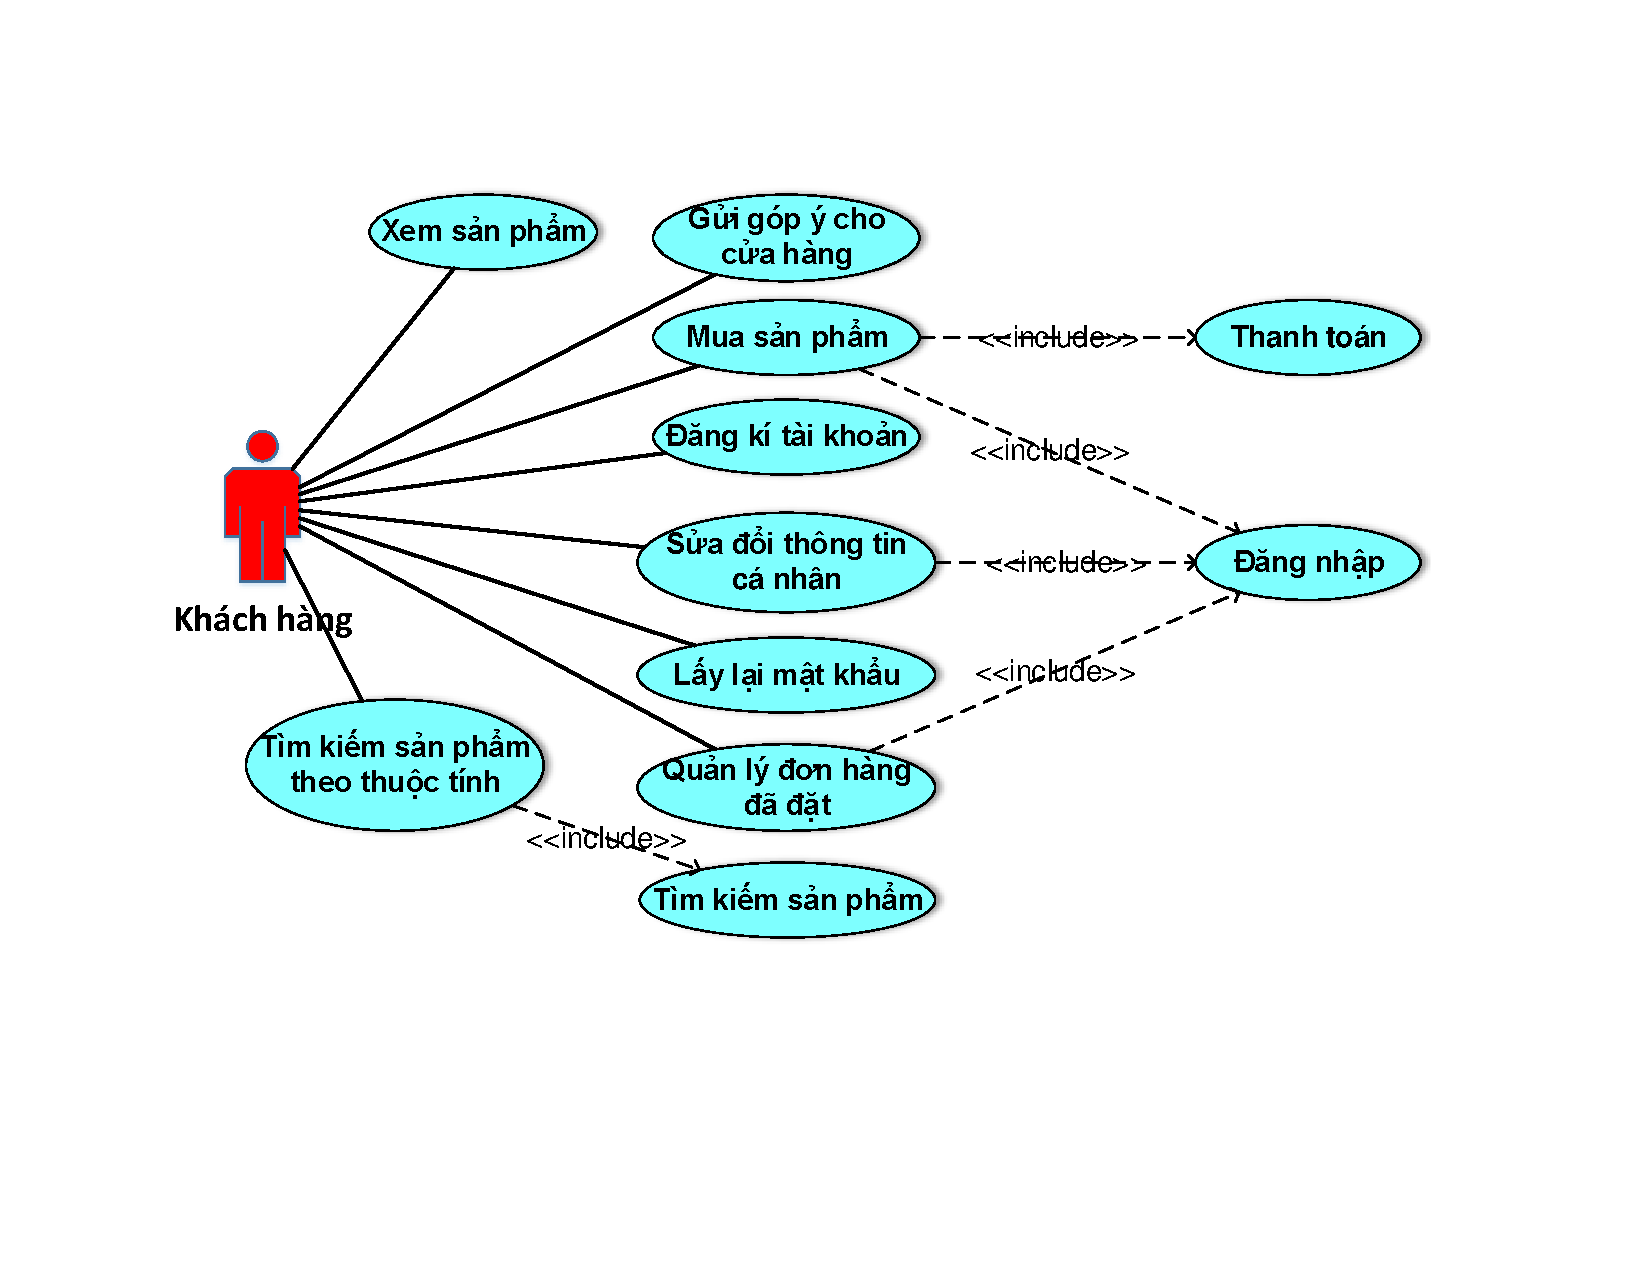
\includegraphics[scale=0.7]{image/UseCaseTongQuanKH.pdf}
    \end{center}
    \caption{Use-Case Khách hàng}
    \label{refhinh3_3}
    \end{figure}
\end{center}
Từ Hình \ref{refhinh3_3} ta có các bảng đặc tả chi tiết cho các Use-Case của khách hàng:
\par
- Use-Case đăng nhập:
\begin{longtable}[htp]{ |m{0.25\linewidth}|m{0.65\linewidth}|}
 \caption{Bảng Use-Case đăng nhập \label{long}}\\
 \hline
 Use-Case & Nội dung \\
 \hline
 Tên Use-Case & Đăng nhập \\
 \hline
 Mô tả & Use-case cho phép khách hàng đăng nhập vào trang chủ để thưc hiện việc mua bán theo như cầu khách hàng\\
 \hline
 Tên tác nhân & Khách hàng\\
 \hline
 Điều kiện kích hoạt & Khách hàng vào trang chủ và nhận nút đăng nhập\\
 \hline
 Tiền điều kiện & Khách hàng đã đăng ký tài khoản trên hệ thống\\
 \hline
 Hậu điều kiện & Khách hàng đăng nhập thành công\\
 \hline
 Luồng sự kiện chính & 
  1. Hệ thống hiện thị màn hình đăng nhập.\newline
  2. Khách hàng nhập tên đăng nhập và mật khẩu.\newline
  3. Hệ thống kiểm tra thông tin đăng nhập.\newline
  4. Nếu thành công hệ thống sẽ đưa khách hàng về trang chủ.\newline
  5. Kết thúc Use-case.	
 \\
 \hline
 Luồng sự kiện phụ & 
 - Tài khoản và mật khẩu không hợp lệ:\newline
 1. Khi khách hàng nhập sai tên đăng nhập và mật khẩu\newline
 2. Hệ thống hiển thị lại màn hình đăng nhập để khách hàng nhập lại thông tin tài khoản và mật khẩu kèm theo thông báo tên đăng nhập và mật khẩu bị sai.\newline
  Quay lại bước 2 trong luồng sự kiện chính.
 \\
 \hline
\end{longtable}
\par
- Use-Case tìm kiếm sản phẩm:
\begin{longtable}[htp]{ |m{0.25\linewidth}|m{0.65\linewidth}|}
 \caption{Bảng Use-Case tìm kiếm sản phẩm \label{long}}\\
 \hline
 Use-Case & Nội dung \\
 \hline
 Tên Use-Case & Tìm kiếm sản phẩm \\
 \hline
 Mô tả & Use-case cho phép khách hàng tìm kiếm các sản phẩm có trong hệ thống theo tên sản phẩm giúp cho khách hàng tiết kiệm thời gian nhất có thể.\\
 \hline
 Tên tác nhân & Khách hàng\\
 \hline
 Điều kiện kích hoạt & Khách hàng truy cập vào trang chủ và nhập dữ liệu cần tìm vào ô tìm kiếm\\
 \hline
 Tiền điều kiện & Khách hàng truy cập vào trang chủ\\
 \hline
 Hậu điều kiện & Tìm kiếm được kết quả về sản phẩm\\
 \hline
 Luồng sự kiện chính & 
  1. Hệ thống hiện thị ô tìm kiếm và yêu cầu người dùng nhập dữ liệu cần tìm kiếm.\newline
  2. Khách hàng nhập dữ liệu cần tìm kiếm.\newline
  3. Hệ thống kiểm tra dữ liệu cần tìm kiếm và sẽ đưa ra gợi ý cho người dùng theo từng kí tự người dùng nhập vào.\newline
  4. Khách hàng lựa chọn 1 sản phẩm đúng theo ý khách hàng dựa trên các gợi ý mà hệ thống đã đưa ra\newline
  5. Kết thúc Use-case.	
 \\
 \hline
 Luồng sự kiện phụ & 
 - Sản phẩm không có trên hệ thống:\newline
 1. Hệ thống kiểm tra theo dữ liệu người dùng nhập vào, dữ liệu người dùng nhập vào không khớp với dữ liệu trong cơ sở dữ liệu hệ thống sẽ hiển thị thông báo không có sản phẩm.\newline
  Quay lại bước 2 trong luồng sự kiện chính.
 \\
 \hline
\end{longtable}

- Use-Case mua sản phẩm:
\begin{longtable}[htp]{ |m{0.25\linewidth}|m{0.65\linewidth}|}
 \caption{Bảng Use-Case mua sản phẩm \label{long}}\\
 \hline
 Use-Case & Nội dung \\
 \hline
 Tên Use-Case & Mua sản phẩm \\
 \hline
 Mô tả & Use-case cho phép khách hàng có thể đặt hàng ngay trên trang chủ.\\
 \hline
 Tên tác nhân & Khách hàng\\
 \hline
 Điều kiện kích hoạt & Khách hàng truy cập vào trang chủ và nhấn vào nút giỏ hàng để tiên hàng đặt hàng \\
 \hline
 Tiền điều kiện & Khách hàng truy cập vào trang chủ và đã đăng nhập vào trang chủ\\
 \hline
 Hậu điều kiện & Thông tin đơn hàng được lưu xuống cơ sở dữ liệu\\
 \hline
 Luồng sự kiện chính & 
  1. Hệ thống hiện thị giao diện đặt hàng và yêu cầu người dùng nhập thông tin đặt hàng.\newline
  2. Khách hàng nhập thông tin đặt hàng .\newline
  3. Hệ thống kiểm tra thông tin đơn hàng và xác nhận hợp lệ.\newline
  4. Hệ thống thông báo đã đặt hàng thành công và đưa khách hàng về trang đơn hàng của tài khoản đang được đăng nhập\newline
  5. Sẽ có điện thoại từ cửa hàng cho khách hàng để xác nhận đơn hàng.
  5. Kết thúc Use-case.	
 \\
 \hline
 Luồng sự kiện phụ & 
 - Khách hàng chưa đăng nhập:\newline
 1.Hệ thống yêu cầu khách hàng đăng nhập trước khi nhấn nút đặt hàng.\newline
  Quay lại bước 1 trong luồng sự kiện chính.
 \\
 \hline
\end{longtable}

-Use-Case thanh toán:
\begin{longtable}[htp]{ |m{0.25\linewidth}|m{0.65\linewidth}|}
 \caption{Bảng Use-Case thanh toán sản phẩm \label{long}}\\
 \hline
 Use-Case & Nội dung \\
 \hline
 Tên Use-Case & Thanh toán sản phẩm \\
 \hline
 Mô tả & Use-case cho phép khách hàng thanh toán trực tuyển các đơn hàng thông qua cổng thanh toán trực tuyển ngân lượng.\\
 \hline
 Tên tác nhân & Khách hàng\\
 \hline
 Điều kiện kích hoạt & Khách hàng truy cập vào trang chủ và nhấn vào nút thanh toán của ngân lượng có trên hoá đơn đặt hàng.\\
 \hline
 Tiền điều kiện & Khách hàng truy cập vào trang chủ đã đăng nhập và có tài khoản ngân lượng với số dự lớn hơn đơn hàng là 2\%.\\
 \hline
 Hậu điều kiện & Nhận được mail thanh toán thành công gửi từ ngân lượng và điện thoại xác nhận từ chủ cửa hàng.\\
 \hline
 Luồng sự kiện chính & 
  1. Khách hàng chọn hoá đơn cần thanh toán trong danh sách hoá đơn mà người dùng đã đặt.
  2. Khách hàng nhấn nút thanh toán để chuyển đến trang giao dịch của ngân lượng.\newline
  3. Khách hàng nhập thông tin tài khoản ngân lượng để tiến hàng giao dịch đơn hàng.\newline
  4. Hệ thông ngân lượng xác nhận lại thông tin đơn hàng.\newline
  5. Khách hàng chọn tiến hàng thanh toán để ngân lượng gửi mã OTP về số điện thoại mà khách hàng đã đăng ký.\newline
  6. Khách hàng nhập mã OTP.\newline 
  7. Hệ thống ngân lượng kiểm tra mã OTP và xác nhận thanh toán.\newline 
  8. Hệ thống ngân lượng sẽ gửi mail cho khách hàng và chủ cửa hàng về thông tin đơn hàng.\newline 
  9. Chủ cửa hàng sẽ xác nhận lại thông tin rồi gọi điện thoại cho khách hàng để chứng thực lại thông tin đơn hàng sau đó sẽ vận chuyển hàng cho khách hàng.\newline 
  5. Kết thúc Use-case.	\newline 
 \\
 \hline
 Luồng sự kiện phụ & 
 - Khách hàng nhập sai tài khoản ngân lượng:\newline
 1. Khi khách hàng nhập sai tên đăng nhập và mật khẩu.\newline
 2. Hệ thống ngân lượng sẽ hiển thị lại màn hình đăng nhập đồng thời hiển thị thông báo đăng nhập không thành công 
  Quay lại bước 3 trong luồng sự kiện chính.
 \\
 \hline
\end{longtable}
\newpage
\subsubsection{Nhân viên quản lý}
\begin{center}
    \begin{figure}[h]
    \begin{center}
     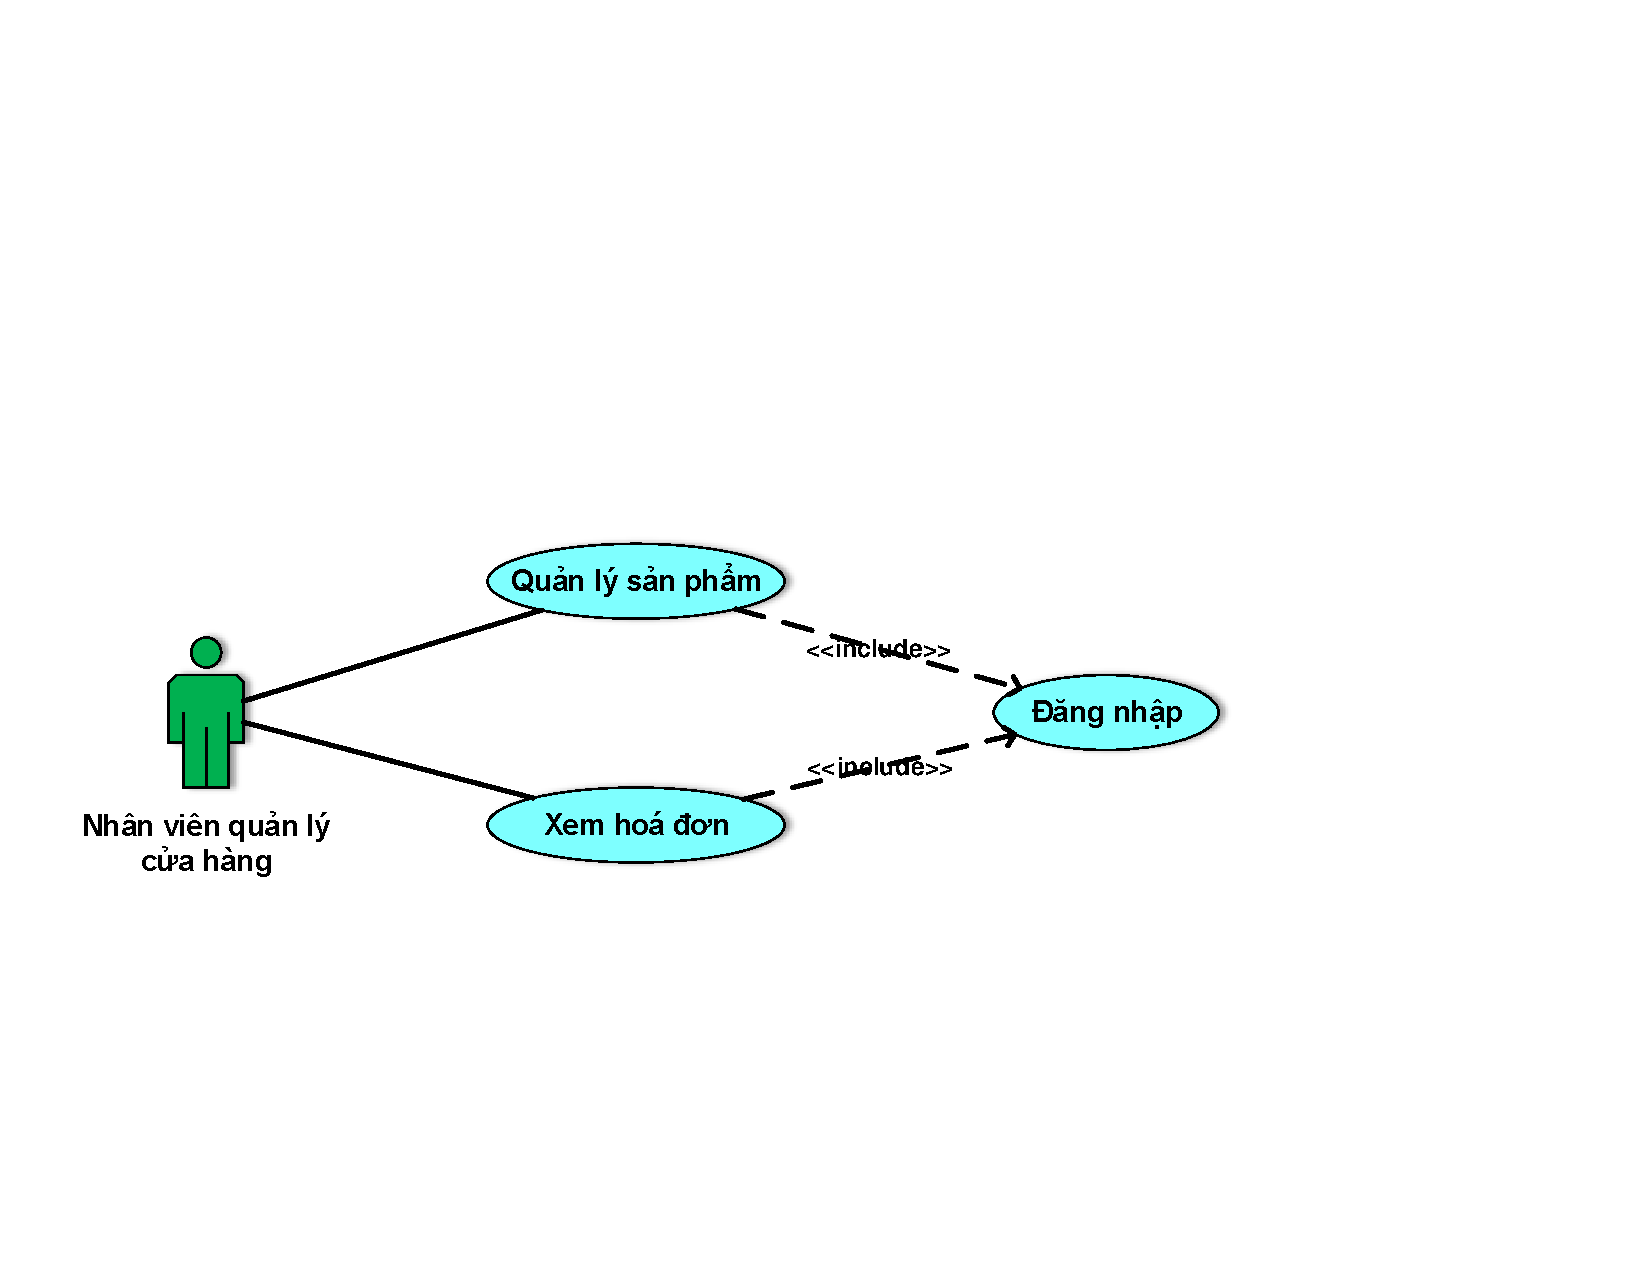
\includegraphics[scale=0.7]{image/UseCaseTongQuanNV.pdf}
    \end{center}
    \caption{Use-Case Nhân viên quản lý}
    \label{refhinh3_4}
    \end{figure}
\end{center}
Hình \ref{refhinh3_4} là use case tổng quan của nhân viên quản lý, nhân viên quản lý trong hệ thống chỉ được phép thêm và xem sản phẩm cũng như xem hoá đơn để xác nhận đơn hàng giúp chủ cửa hàng. Đặc tả chi tiết của use case nhân viên quản lý được thể hiện ở các bảng sau:
\begin{itemize}
\item Đăng nhập được thể hiện ở Bảng \ref{login}
\item Đăng xuất được thể hiện ở Bảng \ref{logout}
\item Thêm sản phẩm được thể hiện ở Bảng \ref{createProduct}
\item Sửa sản phẩm được thể hiện ở Bảng \ref{updateProduct}
\item Xem hoá đơn sản phẩm được thể hiện ở Bảng \ref{listBill}
\end{itemize}
\subsubsection{Người vận chuyển}
\begin{center}
    \begin{figure}[h]
    \begin{center}
     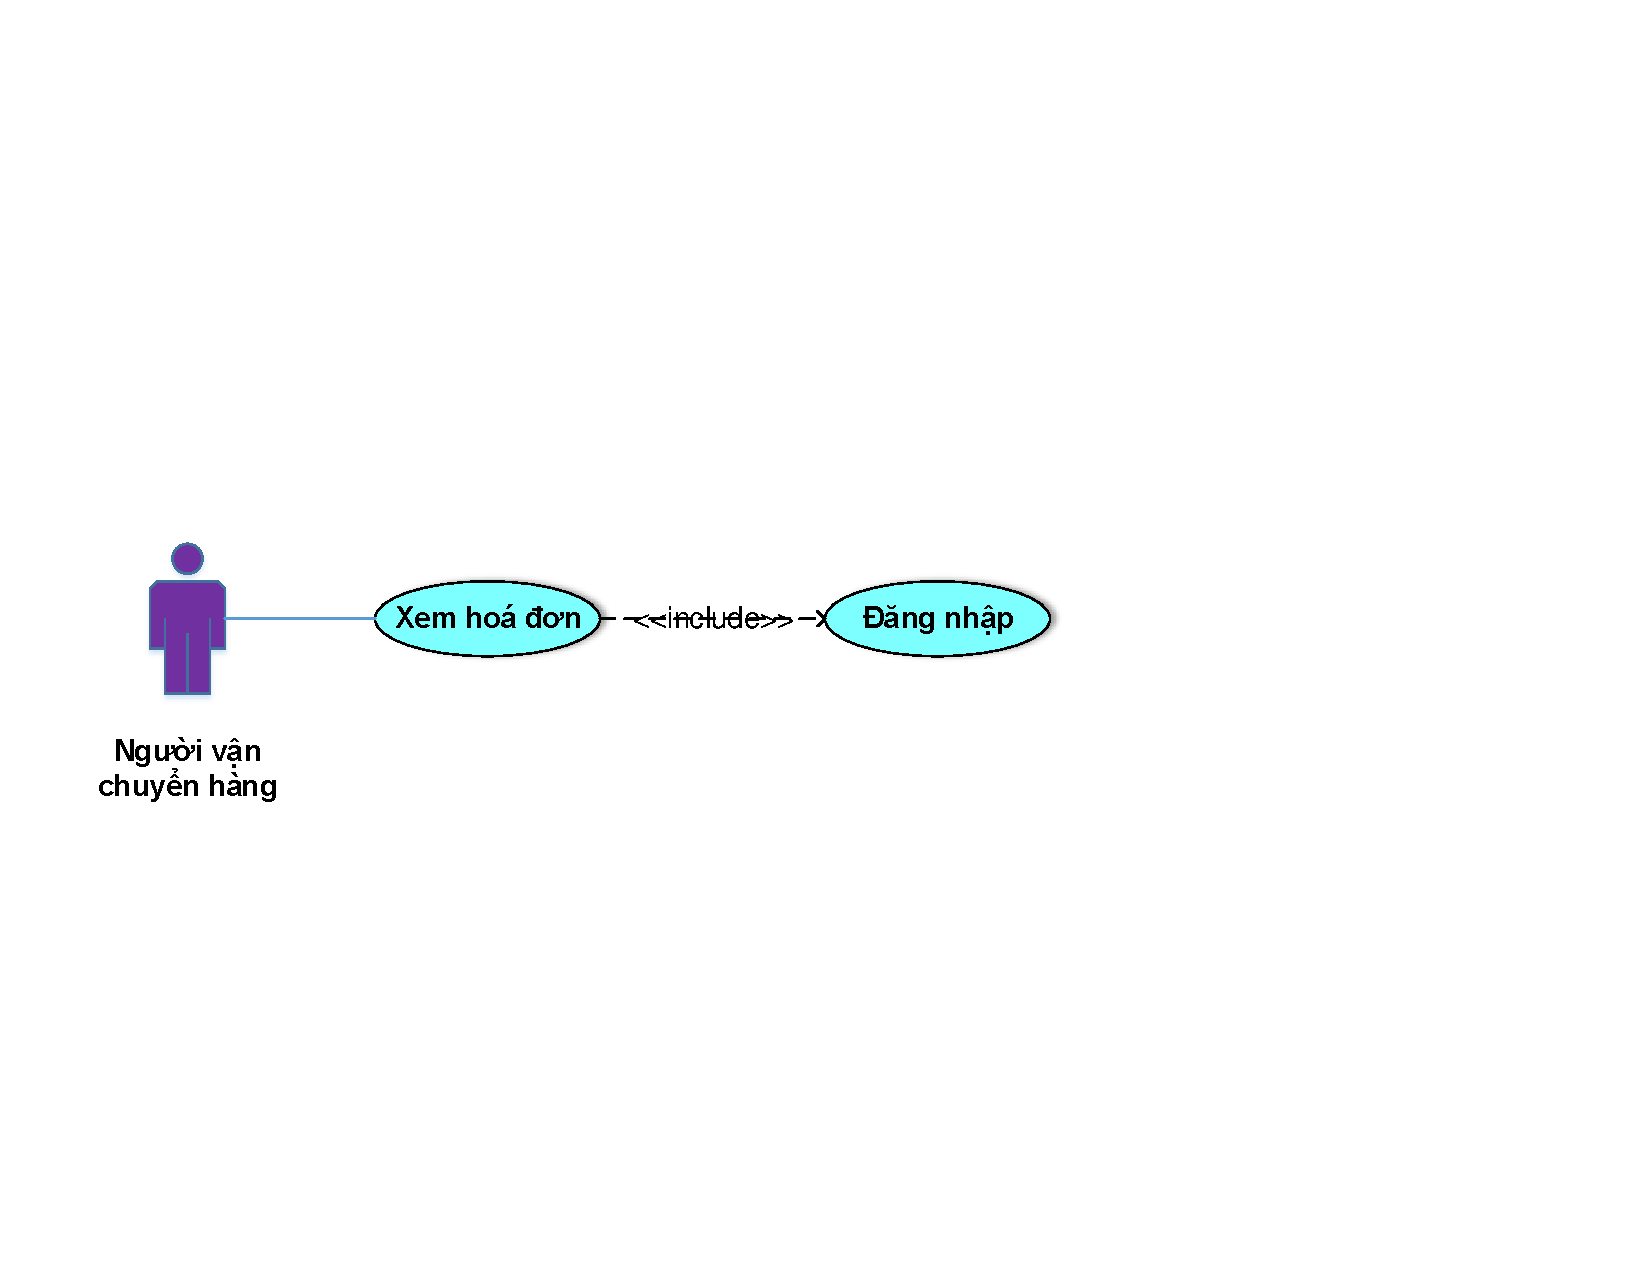
\includegraphics[scale=0.7]{image/UseCaseTongQuanNVC.pdf}
    \end{center}
    \caption{Use-Case Người vận chuyển}
    \label{refhinh3_5}
    \end{figure}
\end{center}
Hình \ref{refhinh3_5} là use case tổng quan của người vận chuyển, người vận chuyển trong hệ thống chỉ được phép xem hoá đơn để xme những đơn hàng nào cần giao hàng. Đặc tả chi tiết của use case người vận chuyển được thể hiện ở các bảng sau:
\begin{itemize}
\item Đăng nhập được thể hiện ở Bảng \ref{login}
\item Đăng xuất được thể hiện ở Bảng \ref{logout}
\item Xem hoá đơn sản phẩm được thể hiện ở Bảng \ref{listBill}
\end{itemize}
\subsection{Biểu đồ tuần tự(sequence diagram)}
Biểu đồ tuần tự minh họa các đối tượng tương tác với nhau ra sao. Chúng tập trung vào các chuỗi thông điệp, có nghĩa là các thông điệp được gửi và nhận giữa một loạt các đối tượng như thế nào. Biểu đồ tuần tự có hai trục: trục nằm dọc chỉ thời gian, trục nằm ngang chỉ ra một tập hợp các đối tượng. Một biểu đồ tuần tự cũng nêu bật sự tương tác trong một kịch bản – một sự tương tác sẽ xảy ra tại một thời điểm nào đó trong quá trình thực thi của hệ thống.
\begin{itemize}
\item Mục đích: biểu diễn tương tác giữa những người dùng và những đối tượng bên trong hệ thống. Biểu đồ này cho biết các thông điệp được truyền tuần tự như thế nào theo thời gian. Thứ tự các sự kiện trong biểu đồ tuần tự hoàn toàn tương tự như trong kịch bản mô tả use case tương ứng.
\item Biểu diễn: Biểu đồ tuần tự được biểu diễn bởi các đối tượng và thông báo truyền đi giữa các đối tượng đó. Trong hệ thống website thương mại điện tử, chúng ta lựa chọn biểu đồ tương tác dạng tuần tự để biểu diễn các tương tác giữa các đối tượng. Để xác định rõ các thành phần cần bổ sung trong biểu đồ lớp, trong mỗi biểu đồ tuần tự của hệ thống quản lý bán hàng sẽ thực hiện:
\begin{itemize}
\item Xác định rõ kiểu của đối tượng tham gia trong tương tác (ví dụ giao diện, điều khiển hay thực thể).
\item Mỗi biểu đồ tuần tự có thể có ít nhất một lớp giao diện tương ứng với chức năng (use case) mà biểu đồ đó mô tả.
\item Mỗi biểu đồ tuần tự có thể liên quan đến một hoặc nhiều đối tượng thực thể. Các đối tượng thực thể chính là các  đối tượng của các lớp  đã được xây dựng trong biểu đồ thiết kế chi tiết.
\end{itemize}
\end{itemize}
\par
Dưới đây là một số biểu đồ tuần tự cho các chức năng của hệ thống quản lý bán hàng:



